% Copyright 2019
% IfV NRW, Fachhochschule Südwestfalen
% Arbeitsgebiet Mediengestaltung und Publishing
%
% Diese Datei wird eingesetzt für die Erstellung von Lerneinheiten im Verbundstudium.

% 2019-10-15
% Sandra Ciupka


\documentclass[paper=a4,fontsize=10pt,pagesize,headsepline=on,oneside,BCOR=13mm,
chapterprefix=false]{scrbook}

\usepackage{includes/ifv}

% Jetzt beginnt das eigentliche Dokument

\begin{document}

	\newgeometry{rmargin=23.5mm,tmargin=29.4mm,textwidth=163mm,textheight=243mm,headheight=8mm}
	
	%\maketitle
	
	\pagestyle{headings}
	\tableofcontents
			
	\restoregeometry
	
	\raggedbottom  % kein einheitlicher Rand unten (-> schönere Abstände zwischen Absätzen)
	\RaggedRight   % Flattersatz mit Trennungen
	
	\begin{spacing}{1.1} % Zeilenabstand
		
		% Copyright 2019
% IfV NRW, Fachhochschule Südwestfalen
% Arbeitsgebiet Mediengestaltung und Publishing
%
% Diese Datei wird eingesetzt für die Erstellung von Lerneinheiten im Verbundstudium.

% 2019-10-15
% Sandra Ciupka


\chapter{Überschrift Vorwort}

Lorem ipsum dolor sit amet, consetetur sadipscing elitr, sed diam nonumy eirmod tempor invidunt ut labore et dolore magna aliquyam erat, sed diam voluptua. At vero eos et accusam et justo duo dolores et ea rebum. Stet clita kasd gubergren, no sea takimata sanctus est Lorem ipsum dolor sit amet. Lorem ipsum dolor sit amet, consetetur sadipscing elitr, sed diam nonumy eirmod tempor invidunt ut labore et dolore magna aliquyam erat, sed diam voluptua. At vero eos et accusam et justo duo dolores et ea rebum. Stet clita kasd gubergren, no sea takimata sanctus est Lorem ipsum dolor sit amet.
\bigskip





	
		% Copyright 2019
% IfV NRW, Fachhochschule Südwestfalen
% Arbeitsgebiet Mediengestaltung und Publishing
%
% Diese Datei wird eingesetzt für die Erstellung von Lerneinheiten im Verbundstudium.

% 2019-10-15
% Sandra Ciupka


\chapter{Überschrift Textebene-1}

Lorem ipsum dolor sit amet, consetetur sadipscing elitr, sed diam nonumy eirmod tempor invidunt ut labore et dolore magna aliquyam erat, sed diam voluptua. At vero eos et accusam et justo duo dolores et ea rebum. Stet clita kasd gubergren, no sea takimata sanctus est Lorem ipsum dolor sit amet. Lorem ipsum dolor sit amet, consetetur sadipscing elitr, sed diam nonumy eirmod tempor invidunt ut labore et dolore magna aliquyam erat, sed diam voluptua. At vero eos et accusam et justo duo dolores et ea rebum. Stet clita kasd gubergren, no sea takimata sanctus est Lorem ipsum dolor sit amet.
\bigskip

Lorem ipsum dolor sit amet, consetetur sadipscing elitr, sed diam nonumy eirmod tempor invidunt ut labore et dolore magna aliquyam erat, sed diam voluptua. At vero eos et accusam et justo duo dolores et ea rebum. Stet clita kasd gubergren, no sea takimata sanctus est Lorem ipsum dolor sit amet. Lorem ipsum dolor sit amet, consetetur sadipscing elitr, sed diam nonumy eirmod tempor invidunt ut labore et dolore magna aliquyam erat, sed diam voluptua. At vero eos et accusam et justo duo dolores et ea rebum. Stet clita kasd gubergren, no sea takimata sanctus est Lorem ipsum dolor sit amet.

%%%%%%%%%%%%%%%%%%%%%%%%%%%%%%%%%%%%%%%%%%%%%%%%%%%%%%%%%%%%%%%%%%%%%%%%%%%%%%%%%%%%%%%%%%%%%%%%%%%%%%%%%%%
\section{Überschrift Textebene-2}

Lorem ipsum dolor sit amet, consetetur sadipscing elitr, sed diam nonumy eirmod tempor invidunt ut labore et dolore magna aliquyam erat, sed diam voluptua. At vero eos et accusam et justo duo dolores et ea rebum. Stet clita kasd gubergren, no sea takimata sanctus est Lorem ipsum dolor sit amet. Lorem ipsum dolor sit amet, consetetur sadipscing elitr, sed diam nonumy eirmod tempor invidunt ut labore et dolore magna aliquyam erat, sed diam voluptua. At vero eos et accusam et justo duo dolores et ea rebum. Stet clita kasd gubergren, no sea takimata sanctus est Lorem ipsum dolor sit amet.

% Abbildung: 107 mm
\begin{figure}[!h]
	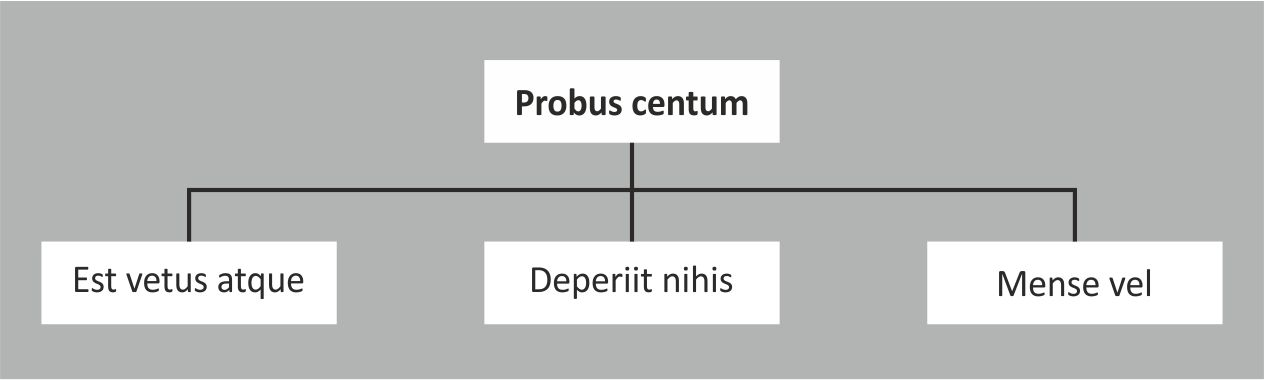
\includegraphics[width=10.7cm]{pics/Abb-001.jpg}
	\caption{Beschriftung einer Abbildung}
	\label{Abb-001}
\end{figure}

%%%%%%%%%%%%%%%%%%%%%%%%%%%%%%%%%%%%%%%%%%%%%%%%%%%%%%%%%%%%%%%%%%%%%%%%%%%%%%%%%%%%%%%%%%%%%%%%%%%%%%%%%%%
\subsection{Überschrift Textebene-3}

Lorem ipsum dolor sit amet, consetetur sadipscing elitr, sed diam nonumy eirmod tempor invidunt ut labore et dolore magna aliquyam erat, sed diam voluptua. At vero eos et accusam et justo duo dolores \mpar{Lorem ipsum} et ea rebum. Stet clita kasd gubergren, no sea takimata sanctus est Lorem ipsum dolor sit amet. Lorem ipsum dolor sit amet, consetetur sadipscing elitr, sed diam nonumy eirmod tempor invidunt ut labore et dolore magna aliquyam erat, sed diam voluptua. At vero eos et accusam et justo duo dolores et ea rebum. Stet clita kasd gubergren, no sea takimata sanctus est Lorem ipsum dolor sit amet.

% Tabelle mit flexiblen Spalten
\begin{table}
	\captionabove{Beschriftung einer Tabelle}
	\begin{tabulary}{10.7cm}{|L|L|L|L|L|L|} % linksbündig
		\hline
		Zelle 1 & 2	& 3 & Zelle 4 & 5 & 6\\
		\hline
		Zelle 7	& 8	& 9 & Zelle 10 & 11 & 12\\
		\hline
	\end{tabulary}
\end{table}



		\chapter{Code Listing}


\begin{listing}[!ht]
\begin{minted}[frame=lines,linenos=true]{python}
import numpy as np
    
def incmatrix(genl1,genl2):
    m = len(genl1)
    n = len(genl2)
    M = None #to become the incidence matrix
    VT = np.zeros((n*m,1), int)  #dummy variable
    
    #compute the bitwise xor matrix
    M1 = bitxormatrix(genl1)
    M2 = np.triu(bitxormatrix(genl2),1) 

    for i in range(m-1):
        for j in range(i+1, m):
            [r,c] = np.where(M2 == M1[i,j])
            for k in range(len(r)):
                VT[(i)*n + r[k]] = 1;
                VT[(i)*n + c[k]] = 1;
                VT[(j)*n + r[k]] = 1;
                VT[(j)*n + c[k]] = 1;
                
                if M is None:
                    M = np.copy(VT)
                else:
                    M = np.concatenate((M, VT), 1)
                
                VT = np.zeros((n*m,1), int)
    
    return M
\end{minted}
\caption{Hello World in C}
\label{listing:2}
\end{listing}

		
	\end{spacing}

%%%%%%%%%%%%%%%%%%%%%%%%%%%%%%%%%%%%%%%%%%%%%%%%%%%%%%%%%%%%%%%%%%%%%%%%%%%%%%%%%%%%%%%%%%%%%%%%%%%%%%%%%
% Abbildungsverzeichnis
% Tabellenverzeichnis

	\listoftables
	\addcontentsline{toc}{section}{Tabellenverzeichnis}
	\listoffigures
	\addcontentsline{toc}{section}{Abbildungsverzeichnis}

%%%%%%%%%%%%%%%%%%%%%%%%%%%%%%%%%%%%%%%%%%%%%%%%%%%%%%%%%%%%%%%%%%%%%%%%%%%%%%%%%%%%%%%%%%%%%%%%%%%%%%%%%
% Klassisches BibTeX

	%\nocite{*}
	%\bibliographystyle{babplain}
	%\bibliographystyle{alphadin} 	% Festlegung Art Zitierung (Havardmethode: Abkuerzung Autor+Jahr)
	
	%Literaturliste soll im Inhaltsverzeichnis auftauchen:
	%\newpage
	%\addcontentsline{toc}{section}{Literaturverzeichnis}
	%\bibliography{Literatur.bib}   % Datei aus Citavi
	
%%%%%%%%%%%%%%%%%%%%%%%%%%%%%%%%%%%%%%%%%%%%%%%%%%%%%%%%%%%%%%%%%%%%%%%%%%%%%%%%%%%%%%%%%%%%%%%%%%%%%%%%% 
% BibLaTeX

	\nocite{*}

	%\newpage
	%\ifkomabibtotocnumbered{true}
	% Copyright 2019
% IfV NRW, Fachhochschule Südwestfalen
% Arbeitsgebiet Mediengestaltung und Publishing
%
% Diese Datei wird eingesetzt für die Erstellung von Lerneinheiten im Verbundstudium.

% 2019-10-15
% Sandra Ciupka


\begin{thebibliography}{}
	\bibitem{Kurzform} Vorname Nachname, Titel, Verlag (Jahr).
\end{thebibliography}


    % Ergänzung angelieferter Daten
	\addcontentsline{toc}{section}{Literaturverzeichnis}
	%\renewcommand\chaptername{\protect Literaturverzeichnis}
	%\printbibliography
	
\end{document}